\documentclass{beamer}
\usetheme[faculty=tw,language=dutch,framenumber,totalframenumber]{UniversiteitGent}
\usepackage{siunitx}

\title{\textbf{Hardware Ontwerpsproject}}
\subtitle{Indoor localisatie voor Drones}
\author{Laurens Bogaert, Thomas Deckmyn \& Zeger Van de Vannet\\Groep 5}

\AtBeginSection[]
{
  \begin{frame}
    \frametitle{Inhoudstafel}
    \tableofcontents[currentsection]
  \end{frame}
}

\usepackage{pifont}

\begin{document}

\begin{frame}
  \titlepage
\end{frame}

\section{Inleiding}
\subsection{Situering}
  \begin{frame}
    \frametitle{Situering}
    GPS:
    \begin{itemize}
        \item Niet voor binnen
        \item Onnauwkeurig (3 m)
        \item Hoogtemeting beperkt
    \end{itemize}
  \end{frame}
  \begin{frame}
    \frametitle{Situering}
    3 onderdelen:
    \begin{itemize}
      \item Algoritmes
      \item Antenne
      \item PCB + Controller
    \end{itemize}
  \end{frame}
\subsection{Planning}
  \begin{frame}
    \frametitle{Planning}
    \begin{tabular}{|l | l | l|}
      \hline
      Week & Titel & Status\\
      \hline
      1 & Toekenning onderwerp & \checkmark\\
      2 & Literatuurstudie \& $1^{ste}$ algoritme & \checkmark\\
      3 & Kennismaking ADS \& $2^{de}$ algoritme & \checkmark\\
      4 - 6 & Antenne design (L \& T) \& PCB-ontwerp (Z) & \checkmark \\
      7 & Afwerking $2^{de}$ algoritme \& Fabricage Antenne (T) & \checkmark \\
       & Vergelijking Algoritmes & \checkmark\\
      8 & Uitmeten Antenne  & \ldots \\
      & Implementatie Microcontroller & \ding{55} \\
      \hline
    \end{tabular}
  \end{frame}
  \begin{frame}
    \frametitle{Planning}
    \begin{verse}
       "Failure is always an option"
    \end{verse}
    \pause
    \begin{itemize}
      \item Redesign Antenne
    \end{itemize}
  \end{frame}
  \begin{frame}
    \frametitle{TODO}
    \begin{itemize}
      \item Solderen PCB
      \item Testen PCB
      \item Implementatie van algoritmes op microcontroller
      \item Integratie
    \end{itemize}
  \end{frame}
\section{PCB Design}
\section{Algoritmes}
\subsection{Ankers}
  \begin{frame}
    \frametitle{Opstelling}
    \begin{figure}
      \begin{center}
        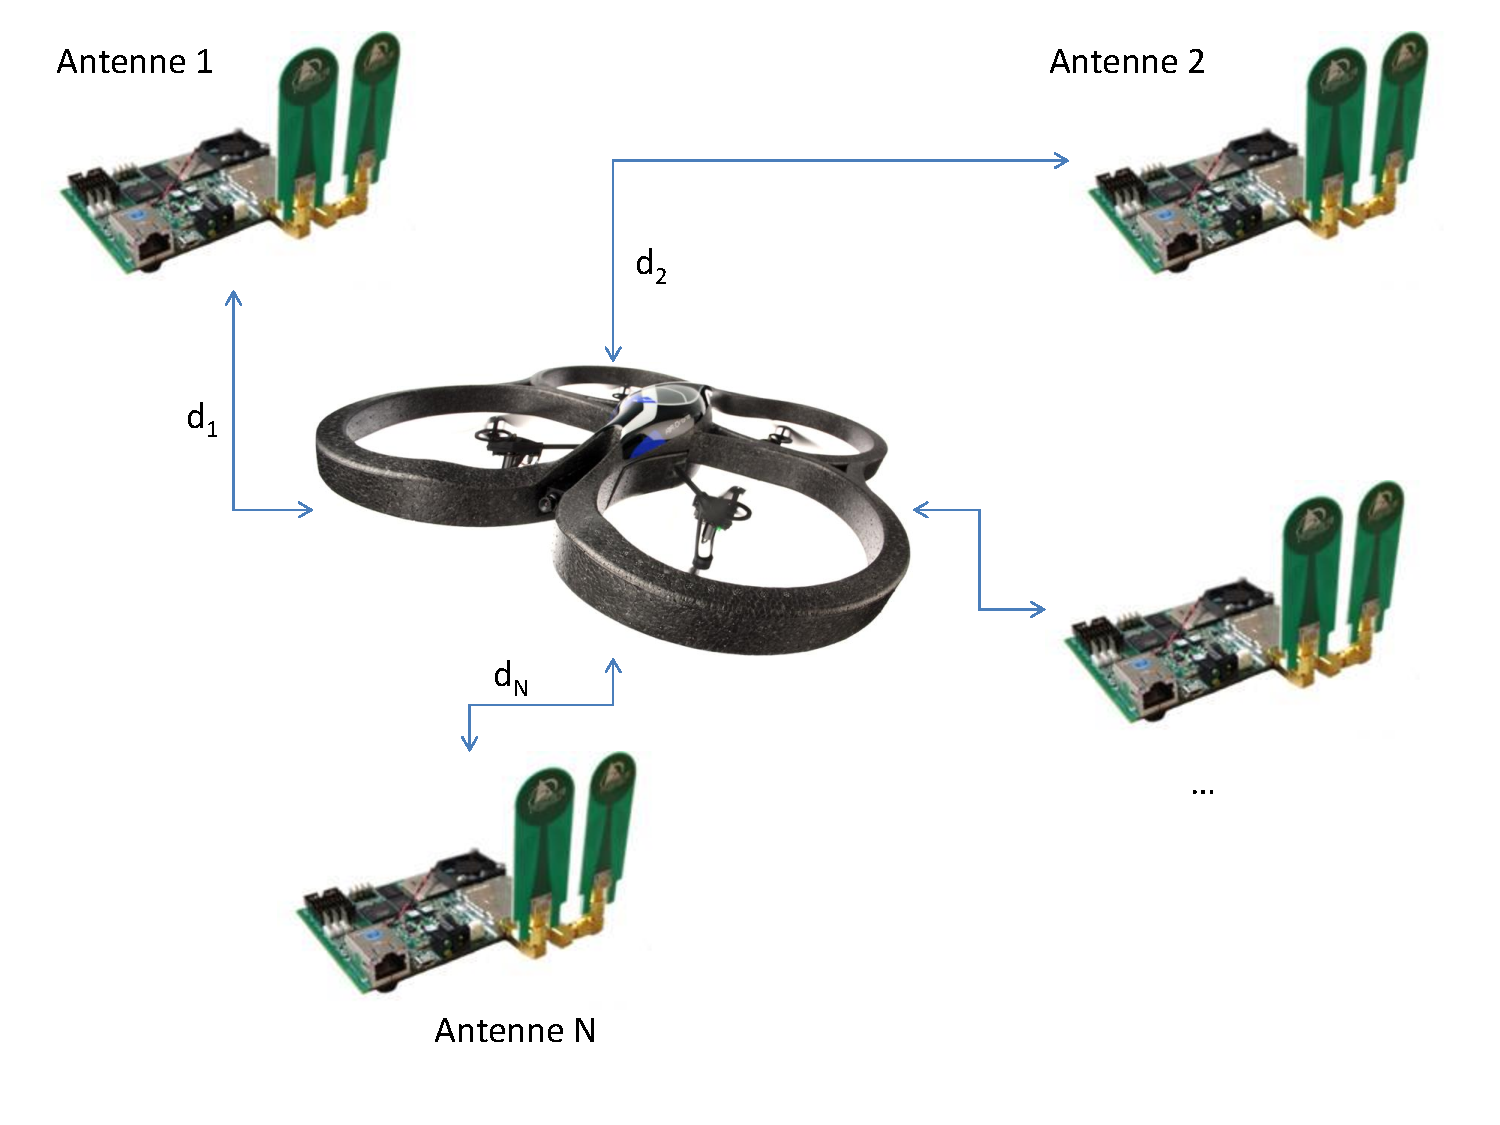
\includegraphics[width=.8\textwidth]{images/opstelling.pdf}
      \end{center}
    \end{figure}
  \end{frame}
  \begin{frame}
    \frametitle{Ankers}
    \begin{itemize}
      \item Gekende positie
      \item Afstand via pulsen $\Rightarrow$ UWB
      \item Meetruis
    \end{itemize}
    \begin{figure}
      \begin{center}
        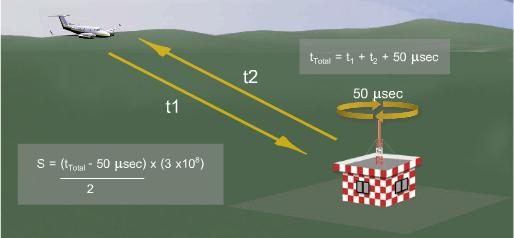
\includegraphics[width=.8\textwidth]{images/DME.jpg}
      \end{center}
    \end{figure}
  \end{frame}
\subsection{Lokalisatie Algoritme}
  \begin{frame}
    \frametitle{Algoritmes}
    \begin{itemize}
      \item LMS: Least Mean Square
      \item Kalman 
    \end{itemize}
  \end{frame}
  \begin{frame}
    \frametitle{Least Mean Square}
    \begin{itemize}
      \item Geen geheugen
        \begin{itemize}
          \item Geen invloed van het verleden
        \end{itemize}
      \item Wat indien er meer vergelijkingen dan onbekenden zijn?
        \begin{itemize}
          \item \# ankers $>$ \# dimensies + 1
          \begin{figure}
            \begin{center}
              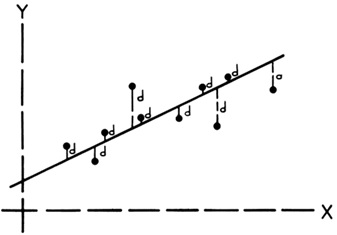
\includegraphics[width=.5\textwidth]{images/LMS.jpg}
            \end{center}
          \end{figure}
        \end{itemize}
    \end{itemize}
  \end{frame}
  \begin{frame}
    \frametitle{Kalman Filter}
    \begin{itemize}
      \item Geheugen $\Rightarrow$ matrices
      \item Bewegingsvrijheid van de drone is beperkt
      \item 2 onderdelen:
        \begin{itemize}
          \item Voorspellen
          \item Meten en updaten
        \end{itemize}
    \end{itemize}
  \end{frame}
  \begin{frame}
    \frametitle{Uitbreiden Kalman Filter}
    \begin{itemize}
      \item Extra Sensoren
        \begin{itemize}
          \item Accelerometer
          \item Gyroscoop
          \item Hoogtemeter
          \item \ldots
        \end{itemize}
      \item Doel: nauwkeuriger volgen
    \end{itemize}
  \end{frame}
\subsection{Resultaten}
  \begin{frame}
    \frametitle{Resultaten: Simulaties}
    % TODO: Afgelegdeweg.jpg (links) en ingezoomd (rechts)
  \end{frame}
  \begin{frame}
    \frametitle{Resultaten: Simulaties}
    % TODO: Cumulatieve errors
  \end{frame}
  \begin{frame}
    \frametitle{LMS vs. Kalman Filter}
    \begin{tabular}{|l|l|}
      \hline
      LMS & Kalman Filter \\
      \hline
      (+) Eenvoudiger & (-) Complexer \\
      (-) Ruwere schatting & (+) Nauwkeuriger \\
      \hline
    \end{tabular}
  \end{frame}
\section{Antenne Ontwerp}
  \begin{frame}
  \frametitle{Referentie Antenne}
  \begin{columns}[c]
  \begin{column}{0.5\textwidth}
    \begin{itemize}
      \item BroadSpec\texttrademark  UWB Antenne 
      \item Omnidirectioneel in azimuth
      \item Ontwerpsparameters:
      \begin{itemize}
        \item $\SI{3.1}{\giga\hertz}$ - $\SI{5.3}{\giga\hertz}$
        \item Gain nominaal $\approx \SI{3}{\decibel}$ 
        \item Lineaire fase respons
        \item Efficientie $\approx$ 90\%
      \end{itemize}
    \end{itemize}
    \end{column}

    \begin{column}{0.5\textwidth}
    \centering
      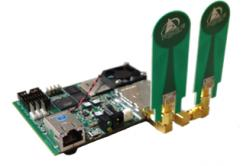
\includegraphics[width=0.7\textwidth]{images/Pulson400UWB.jpg}
    \end{column}
    \end{columns}

  \end{frame}

  \begin{frame}
  \frametitle{Antenne Ontwerp}
  \begin{itemize}
    \item Start: Rechthoekige Patch Antenne
      \begin{itemize}
        \item Lengte: Resonantie frequentie $f_0 = \SI{4.2}{\mega\hertz}$
              \begin{align}  L = \frac{c}{2 f_r \sqrt{\epsilon_r}}  \nonumber \end{align}
        \item Breedte: \begin{align} \text{Uitgestraald vermogen} \nonumber & \implies \text{Resonantie weerstand} \downarrow \\ & \implies \text{Bandbreedte} \uparrow, \text{Efficiency} \uparrow \nonumber \end{align}

      \end{itemize}
    \item Dimensies drone! $\implies$ Andere manier BW $\uparrow$ 
    \end{itemize}
  \end{frame}

  \begin{frame}
  \frametitle{Antenne Ontwerp}
  
  \begin{columns}[c]
  \begin{column}{0.5\textwidth}
    \begin{itemize}
      \item Toevoegen \textit{Trap} $\implies$ BW $\uparrow$
      \item Partieel grondvlak
      \begin{itemize}
        \item Optimaliseren dimensies \begin{align} & \implies \text{Vlakke } S_{11} \nonumber \\ & \implies \text{Lineaire fase} \nonumber \end{align}
      \end{itemize}

    \end{itemize}
  \end{column}

  \begin{column}{0.5\textwidth}
  \centering
    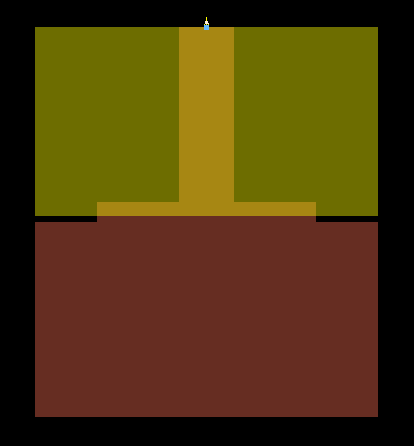
\includegraphics[width=0.7\textwidth]{images/antenne_ontwerp.png}
  \end{column}
  \end{columns}
  \end{frame}

  \begin{frame}
  \frametitle{Simulatie Antenne}

  \end{frame}

\end{document}
